\section{Experimental Results}
\label{sec:exp_results}
\subsection{Single Teacher vs Multi teacher}

% \begin{table*}[!h]
%     \centering
%     \begin{tabular}{ccccccccccc}
%         \toprule
%         \multirow{2}{*}{Model ID} & \multicolumn{3}{c}{Teacher Models} & \multirow{2}{*}{Embedding KD}& \multirow{2}{*}{nBest KD} & \multicolumn{2}{c}{dev}   & \multicolumn{2}{c}{test}\\
%         \cmidrule(lr){2-4} \cmidrule(lr){7-8}  \cmidrule(lr){9-10}
%         & w2v2& Hu & WavLM & & & \multicolumn{1}{c}{clean} & \multicolumn{1}{c}{other} & \multicolumn{1}{c}{clean} & \multicolumn{1}{c}{other}  \\
%         \midrule
%         Baseline & - & - & - & - & - & 7.5 & 20.9 & 8.0 & 21.8 \\
%         \midrule
%         \multirow{6}{*}{Single teacher} & \cmark &   &   & \cmark & & 6.8 & 20.9 & 7.2 & 21.7\\
%         &   & \cmark &   & \cmark & & 6.7 & 20.5 & 7.0 & 21.2\\
%         &   &   & \cmark & \cmark & & 6.5 & 20.2 & 6.7 & 20.7\\
%         & \cmark &   &   & \cmark & \cmark & 6.6 & 20.7 & 6.8 & 20.9\\
%         &   & \cmark &   & \cmark & \cmark & 6.6 & 20.3 & 6.8 & 20.7\\
%         &   &   & \cmark & \cmark & \cmark & \textbf{6.5} & \textbf{20.1} & \textbf{6.6} & \textbf{20.6}\\
        
%         \midrule
%         \multirow{6}{*}{Multi teacher} & \cmark & \cmark &   & \cmark & & 6.4 & 19.6 & 6.6 & 20.0 \\
%         & \cmark & \cmark &   & & \cmark & 6.4 & 19.6 & 6.6 & 20.0 \\
%         & \cmark & \cmark &   & \cmark & \cmark & 6.4 & 19.6 & 6.6 & 20.0 \\
%         &   & \cmark & \cmark & & \cmark & 6.2 & 19.2 & 6.6 & 19.5\\
%         &   & \cmark & \cmark & \cmark & & 6.2 & 19.2 & 6.6 & 19.5\\
%         &   & \cmark & \cmark & \cmark & \cmark & 6.2 & 19.2 & 6.6 & 19.5\\
%         \bottomrule
%     \end{tabular}
%     \caption{Caption}
%     \label{tab:my_label}
% \end{table*}

% \begin{table}[!h]
%     \centering
%     \begin{tabular}{lcccc}
%         \toprule
%         \multirow{2}{*}{Transducer models}    & \multicolumn{2}{c}{dev}   & \multicolumn{2}{c}{test}  \\
%         \cmidrule(lr){2-3}  \cmidrule(lr){4-5}
%         & \multicolumn{1}{c}{clean} & \multicolumn{1}{c}{other} & \multicolumn{1}{c}{clean} & \multicolumn{1}{c}{other} \\ 
%         \midrule
%         \multicolumn{5}{l}{\textbf{Reference models: 100h}}\\
%         % W2v2 transducer & 5.1 & 12.2 & 5.2 & 11.8\\
%         % Hubert transducer    & 5.2 & 11.0 & 5.3 & 11.2 \\
%         % WavLM base+ transducer & 3.9 & 8.4 & 3.9 & 8.3 \\
%         Conformer-S, baseline    & 7.5 & 20.9 & 8.0 & 21.8 \\
%         \midrule
%         \multicolumn{5}{l}{\textbf{Single teacher}}\\
%         W2v2, init & 6.8 & 20.9 & 7.2 & 21.7\\
%         W2v2, init+1Best & 6.6 & 20.7 & 6.8 & 20.9\\
        
%         Hubert, init & 6.7 & 20.5 & 7.0 & 21.2 \\
%         Hubert, init+1Best & 6.6 & 20.3 & 6.8 & 20.7 \\
        
%         WavLM, init & 6.5 & 20.2 & 6.7 & 20.7\\
%         WavLM, init+1Best & \textbf{6.5} & \textbf{20.1} & \textbf{6.6} & \textbf{20.6} \\
        
%         \midrule
%         \multicolumn{5}{l}{\textbf{Multi teacher}}\\
%         W2v2+Hu, 2Best & 6.6 & 19.0 & 6.9 & 19.4 \\
%         W2v2+Hu, init  & 6.4 & 19.6 & 6.6 & 20.0 \\
%         W2v2+Hu, init+2Best & 6.2 & 19.2 & 6.5 & 19.4\\
        
%         WavLM+Hu, 2Best & 6.6 & 19.0 & 6.8 & 19.3 \\
%         WavLM+Hu  & 6.2 & 19.2 & 6.6 & 19.5 \\
%         WavLM+Hu, init+2Best & \textbf{6.1} & \textbf{18.9} & \textbf{6.5} & \textbf{19.2} \\
        
%         \bottomrule
%     \end{tabular}
%     \caption{\%WERs for non-streaming student transducer models. ``Hu'' stands for HuBERT and ``W2v2'' stands for Wav2vec 2.0.}
%     \label{tab:feature kd 100h}
% \end{table}

% \begin{table}[!h]
%     \centering
%     \begin{adjustbox}{width=\linewidth}
%     \begin{tabular}{lcccccccc}
%         \toprule
%         \multicolumn{3}{c}{Teacher Models} & \multicolumn{2}{c}{KD}  & \multicolumn{2}{c}{dev}   & \multicolumn{2}{c}{test}  \\
%         \cmidrule(lr){1-3} \cmidrule(lr){4-5} \cmidrule(lr){6-7} \cmidrule(lr){8-9}
%         \multicolumn{1}{c}{W2v2} & \multicolumn{1}{c}{Hu} & \multicolumn{1}{c}{WL} &\multicolumn{1}{c}{Embedding} & \multicolumn{1}{c}{nBest} & \multicolumn{1}{c}{clean} & \multicolumn{1}{c}{other} & \multicolumn{1}{c}{clean} & \multicolumn{1}{c}{other} \\ 
%         \midrule
%         \multicolumn{5}{l}{\textbf{Baseline 100h, Non-streaming}}\\
%         % W2v2 transducer & 5.1 & 12.2 & 5.2 & 11.8\\
%         % Hubert transducer    & 5.2 & 11.0 & 5.3 & 11.2 \\
%         % WavLM base+ transducer & 3.9 & 8.4 & 3.9 & 8.3 \\
%          - & - & - & - & - & 7.5 & 20.9 & 8.0 & 21.8 \\
%         \midrule
%         \multicolumn{5}{l}{\textbf{Single teacher}}\\
%         \checkmark &  & & \checkmark & & 6.8 & 20.9 & 7.2 & 21.7\\
%         \checkmark &  & & \checkmark & \checkmark & 6.6 & 20.7 & 6.8 & 20.9\\
        
%         & \checkmark &  & \checkmark & & 6.7 & 20.5 & 7.0 & 21.2 \\
%         & \checkmark &  & \checkmark & \checkmark & 6.6 & 20.3 & 6.8 & 20.7 \\
        
%         &  & \checkmark & \checkmark &  & 6.5 & 20.2 & 6.7 & 20.7\\
%         &  & \checkmark & \checkmark & \checkmark & \textbf{6.5} & \textbf{20.1} & \textbf{6.6} & \textbf{20.6} \\
        
%         \midrule
%         \multicolumn{5}{l}{\textbf{Multi teacher}}\\
%         \checkmark & \checkmark &  & & \checkmark & 6.6 & 19.0 & 6.9 & 19.4 \\
%         \checkmark & \checkmark & & \checkmark &  & 6.4 & 19.6 & 6.6 & 20.0 \\
%         \checkmark & \checkmark & & \checkmark & \checkmark  & 6.2 & 19.2 & 6.5 & 19.4\\
        
%         %WavLM+Hu & & \checkmark & 6.6 & 19.0 & 6.8 & 19.3 \\
%         & \checkmark & \checkmark & & \checkmark & 6.6 & 19.0 & 6.8 & 19.3 \\
%         & \checkmark &\checkmark  & \checkmark & &6.2 & 19.2 & 6.6 & 19.5 \\
%         & \checkmark & \checkmark & \checkmark & \checkmark & \textbf{6.1} & \textbf{18.9} & \textbf{6.5} & \textbf{19.2} \\
        
%         \bottomrule
%     \end{tabular}
%     \end{adjustbox}
%     \caption{\%WERs for non-streaming student transducer models. A tick under embedding KD means that embedding-level encoder pretraininng is used. A tick under nBest KD means either 1-best or n-best KD is adopted depending on the number of teachers. ``W2v2'', ``Hu'' and ``WL'' stand for Wav2vec 2.0, HuBERT and WavLM respectively. }
%     \label{tab:feature kd 100h}
% \end{table}

\begin{table}[!ht]
    \centering
    \begin{adjustbox}{width=\linewidth}
    \begin{tabular}{lcccccc}
        \toprule
        \multirow{2}{*}{\shortstack[c]{Teacher\\model}} & \multicolumn{2}{c}{KD}  & \multicolumn{2}{c}{dev}   & \multicolumn{2}{c}{test}  \\
        \cmidrule(lr){2-3} \cmidrule(lr){4-5} \cmidrule(lr){6-7} 
         &\multicolumn{1}{c}{Embedding} & \multicolumn{1}{c}{nBest} & \multicolumn{1}{c}{clean} & \multicolumn{1}{c}{other} & \multicolumn{1}{c}{clean} & \multicolumn{1}{c}{other} \\ 
        \midrule
        \multicolumn{5}{l}{\textbf{Non-streaming baseline, no KD}}\\
        % W2v2 transducer & 5.1 & 12.2 & 5.2 & 11.8\\
        % Hubert transducer    & 5.2 & 11.0 & 5.3 & 11.2 \\
        % WavLM base+ transducer & 3.9 & 8.4 & 3.9 & 8.3 \\
        -  & - & - & 7.5 & 20.9 & 8.0 & 21.8 \\
        \midrule
        \multicolumn{5}{l}{\textbf{Single teacher KD}} \\
        W2v2 & \checkmark &  & 6.8 & 20.9 & 7.2 & 21.7 \\
        W2v2 & \checkmark & \checkmark & 6.6 & 20.7 & 6.8 & 20.9\\
        
        Hu& \checkmark & & 6.7 & 20.5 & 7.0 & 21.2 \\
        Hu& \checkmark & \checkmark & 6.6 & 20.3 & 6.8 & 20.7 \\
        
        WL & \checkmark &  & 6.5 & 20.2 & 6.7 & 20.7\\
        WL & \checkmark & \checkmark & \textbf{6.5} & \textbf{20.1} & \textbf{6.6} & \textbf{20.6} \\
        
        \midrule
        \multicolumn{5}{l}{\textbf{Multi teacher KD}}\\
        W2v2+Hu & & \checkmark & 6.6 & 19.0 & 6.9 & 19.4 \\
        W2v2+Hu & \checkmark &  & 6.4 & 19.6 & 6.6 & 19.8 \\
        W2v2+Hu & \checkmark & \checkmark  & 6.2 & 19.2 & 6.5 & 19.4\\
        
        %WavLM+Hu & & \checkmark & 6.6 & 19.0 & 6.8 & 19.3 \\
        WL+Hu & & \checkmark & 6.6 & 19.0 & 6.8 & 19.3 \\
        WL+Hu  & \checkmark & &6.2 & 19.2 & 6.6 & 19.5 \\
        WL+Hu & \checkmark & \checkmark & \textbf{6.1} & \textbf{18.9} & \textbf{6.5} & \textbf{19.2} \\
        
        \bottomrule
    \end{tabular}
    \end{adjustbox}
    \caption{\%WERs for non-streaming student transducer models. A tick under embedding KD or n-best KD means that embedding-level encoder pretraininng or 1-best (or n-best if multiple teachers are used) is adopted. ``W2v2'', ``Hu'' and ``WL'' stand for Wav2vec 2.0, HuBERT and WavLM respectively.}
    \label{tab:feature kd 100h}
\end{table}

Experiments were first carried out on the "train-clean-100" subset. Results on non-streaming transducers are reported in \tbl{feature kd 100h}. The following observations can be made. First, using encoder embeddings from self-supervised pre-trained models for KD successfully improves the performance of the student model. Second, the performance of the student model after embedding-level KD training is better when the teacher model has lower WERs. The best performing student model under single teacher setup is pre-trained using embeddings extracted from WavLM, which is also the best among the three teacher models, achieving 16.2\% and 5.0\% relative WERR on the test sets compared to the baseline model. Third, increasing the number of teachers leads to a further WER reduction. By using a teacher combination of HuBERT and WavLM during encoder pre-training, further relative WERRs of 1.5\% and 4.6\% is achieved compared to the best single-teacher setup. Fourth, embedding level KD is compatible with n-best alignment-based KD for both the single-teacher and multi-teacher setups. Larger WER reductions are observed after adding n-best alignment KD loss to the HuBERT+WavLM setup, leading to final relative WERRs of 18.8\% and 11.9\% compared to the baseline. Note that the performance improvement on test-clean is bigger than on the more challenging test-other set. This could be the reason that the student model is only pre-trained on the train-clean-100 subset, which is more acoustically similar to test-clean.
%After combining n-best KD The best setup is combining embedding level KD with n-best alignment KD using HuBERT and WavLM as teacher model at the same time.

Experiments are then carried out for streaming student transducer models. Results in the 100-hour setup are shown in \tbl{feature kd streaming 100h}. To verify the effectiveness of $\tau$, student models trained with different $\tau$ values were compared under the single-teacher setup. It can be seen that $\tau=7$ consistently outperforms $\tau=0$ (which is equivalent to allowing no delay in the streaming student model), suggesting the necessity of choosing a sensible $\tau$ value during embedding level KD for streaming student model. The model trained with $\tau=0$ even performs worse than the baseline model trained without distillation. Therefore, $\tau$ is set to 7 in the following experiments. When combined with 1-best KD in the second stage, the same $\tau=7$ used during encoder pre-training was adopted when using \eqndot{1best alignment streaming} for one-best loss computation. Similar trends as in \tbl{feature kd 100h} can be observed for streaming student models. Using embedding-level KD consistently improves the student model under the single-teacher setup and a further gain is observed when two teachers are used for encoder pre-training or adding n-best alignment KD during fine-tuning. The best streaming student model is obtained under the two-teacher embedding KD setup with HuBERT and WavLM combined with 2-best KD during self-supervised fine-tuning, resulting in relative WERRs of 19.7\% and 7.8\% compared to the baseline model trained without KD. 

% \begin{table}[!h]
%     \centering
%     \begin{tabular}{lcccc}
%         \toprule
%          \multirow{2}{*}{Transducer models}    & \multicolumn{2}{c}{dev}   & \multicolumn{2}{c}{test}  \\
%         \cmidrule(lr){2-3}  \cmidrule(lr){4-5}
%         & \multicolumn{1}{c}{clean} & \multicolumn{1}{c}{other} & \multicolumn{1}{c}{clean} & \multicolumn{1}{c}{other} \\ 
%         \midrule
%         Conformer-S, baseline    & 11.2 & 28.4 & 12.2 & 29.6 \\
%         \midrule
%         \multicolumn{5}{l}{\textbf{Single teacher}} \\
%         W2v2, $\tau=0$ & 10.4 & 28.8 & 11.1 & 30.0 \\
%         W2v2, $\tau=7$ & 10.0 & 27.6 & 10.2 & 28.6 \\
%         Hu, $\tau=0$ & 10.4 & 28.6 & 11.0 & 29.9 \\
%         Hu, $\tau=7$ & 9.9 & 27.4 & 10.2 & 28.5 \\
%         WavLM, $\tau=0$ & 10.3 & 28.3 & 10.8 & 29.4\\
%         WavLM, $\tau=7$ & 9.8 & 27.2 & 10.1 & 28.2 \\
%         \bottomrule
%     \end{tabular}
%     \caption{Comparison between two different $\tau$ for student models trained with a single teacher.}
%     \label{tab:my_label}
% \end{table}

\begin{table}[!ht]
    \centering
    \begin{adjustbox}{width=\linewidth}
    \begin{tabular}{lcccccc}
        \toprule
        \multirow{2}{*}{\shortstack[c]{Teacher\\model}} & \multicolumn{2}{c}{KD}  & \multicolumn{2}{c}{dev}   & \multicolumn{2}{c}{test}  \\
        \cmidrule(lr){2-3} \cmidrule(lr){4-5} \cmidrule(lr){6-7} 
         &\multicolumn{1}{c}{Embedding} & \multicolumn{1}{c}{nBest} & \multicolumn{1}{c}{clean} & \multicolumn{1}{c}{other} & \multicolumn{1}{c}{clean} & \multicolumn{1}{c}{other} \\ 
        \midrule
        \multicolumn{5}{l}{\textbf{Streaming baseline, no KD}}\\
        % W2v2 transducer & 5.1 & 12.2 & 5.2 & 11.8\\
        % Hubert transducer    & 5.2 & 11.0 & 5.3 & 11.2 \\
        % WavLM base+ transducer & 3.9 & 8.4 & 3.9 & 8.3 \\
        - & - & - & 11.2 & 28.4 & 12.2 & 29.6 \\
        \midrule
        \multicolumn{5}{l}{\textbf{Single teacher KD}} \\
        W2v2, $\tau=0$ & \checkmark &  & 10.4 & 28.8 & 11.1 & 30.0 \\
        W2v2 & \checkmark &  & 9.9 & 27.4 & 10.2 & 28.5\\
        W2v2 & \checkmark & \checkmark & 9.9 & 27.4 & 10.1 & 28.4 \\
        
        Hu, $\tau=0$& \checkmark &  & 10.4 & 28.6 & 11.0 & 29.9 \\
        Hu &\checkmark & & 9.9 & 27.4 & 10.2 & 28.5 \\
        Hu &\checkmark & \checkmark & 9.9 & 27.1 & 10.1 & 28.3 \\
        
        WL, $\tau=0$ & \checkmark &  & 10.3 & 28.3 & 10.8 & 29.4\\
        WL & \checkmark &  & 9.8 & 27.2 & 10.1 & 28.2\\
        WL & \checkmark & \checkmark &  \textbf{9.7} & \textbf{26.9} & \textbf{10.1} & \textbf{28.0}  \\
        
        \midrule
        \multicolumn{5}{l}{\textbf{Multi teacher KD}}\\
        
        W2v2+Hu & \checkmark &  & 9.7 & 26.9 & 10.0 & 27.9 \\
        W2v2+Hu & \checkmark & \checkmark  & 9.6 & 26.8 & 9.9 & 27.7\\
        
        WL+Hu  & \checkmark & & 9.6 & 26.6 & 9.9 & 27.6 \\
        WL+Hu & \checkmark & \checkmark & \textbf{9.5} & \textbf{26.4} & \textbf{9.8} & \textbf{27.3} \\
        
        \bottomrule
    \end{tabular}
    \end{adjustbox}
    \caption{\%WERs for streaming student transducer models. $\tau$ is the time-shift factor used during embedding KD and is set to 7 unless explicitly specified.}
    \label{tab:feature kd streaming 100h}
\end{table}
\posttbl


% \begin{table}[!h]
%     \centering
%     \begin{adjustbox}{width=\linewidth}
%     \begin{tabular}{lccccccc}
%         \toprule
%         \multirow{2}{*}{Model ID} & \multirow{2}{*}{$\tau$} & \multicolumn{2}{c}{KD}  & \multicolumn{2}{c}{dev}   & \multicolumn{2}{c}{test}  \\
%         \cmidrule(lr){3-4} \cmidrule(lr){5-6} \cmidrule(lr){7-8} 
%          & & \multicolumn{1}{c}{Embedding} & \multicolumn{1}{c}{nBest} & \multicolumn{1}{c}{clean} & \multicolumn{1}{c}{other} & \multicolumn{1}{c}{clean} & \multicolumn{1}{c}{other} \\ 
%         \midrule
%         \multicolumn{5}{l}{\textbf{No KD, streaming}}\\
%         % W2v2 transducer & 5.1 & 12.2 & 5.2 & 11.8\\
%         % Hubert transducer    & 5.2 & 11.0 & 5.3 & 11.2 \\
%         % WavLM base+ transducer & 3.9 & 8.4 & 3.9 & 8.3 \\
%          - & - & - & - & 11.2 & 28.4 & 12.2 & 29.6 \\
%         \midrule
%         \multicolumn{5}{l}{\textbf{Single teacher KD}} \\
%         W2v2 & 0 &\checkmark &  & 10.4 & 28.8 & 11.1 & 30.0 \\
%         W2v2 & 7 &\checkmark &  & 9.9 & 27.4 & 10.2 & 28.5\\
%         W2v2 & 7 &\checkmark & \checkmark & 9.9 & 27.4 & 10.1 & 28.4 \\
        
%         Hu& 0 &\checkmark &  & 10.4 & 28.6 & 11.0 & 29.9 \\
%         Hu& 7 &\checkmark & & 9.9 & 27.4 & 10.2 & 28.5 \\
%         Hu& 7 &\checkmark & \checkmark & 9.9 & 27.1 & 10.1 & 28.3 \\
        
%         WL & 0 &\checkmark &  & 10.3 & 28.3 & 10.8 & 29.4\\
%         WL & 7 &\checkmark &  & 9.8 & 27.2 & 10.1 & 28.2\\
%         WL & 7 &\checkmark & \checkmark &  \textbf{9.7} & \textbf{26.9} & \textbf{10.1} & \textbf{28.0}  \\
        
%         \midrule
%         \multicolumn{5}{l}{\textbf{Multi teacher KD}}\\
        
%         W2v2+Hu & 7 &\checkmark &  & 6.4 & 19.6 & 6.6 & 20.0 \\
%         W2v2+Hu & 7 &\checkmark & \checkmark  & 6.2 & 19.2 & 6.5 & 19.4\\
        
%         WavLM+Hu  & 7 &\checkmark & &6.2 & 19.2 & 6.6 & 19.5 \\
%         WavLM+Hu & 7 &\checkmark & \checkmark & \textbf{6.1} & \textbf{18.9} & \textbf{6.5} & \textbf{19.2} \\
        
%         \bottomrule
%     \end{tabular}
%     \end{adjustbox}
%     \caption{\%WERs for streaming student transducer models. }
%     \label{tab:feature kd 100h}
% \end{table}

% \begin{table}[!h]
%     \centering
%     \begin{tabular}{lcccc}
%         \toprule
%         \multirow{2}{*}{Transducer models}    & \multicolumn{2}{c}{dev}   & \multicolumn{2}{c}{test}  \\
%         \cmidrule(lr){2-3}  \cmidrule(lr){4-5}
%         & \multicolumn{1}{c}{clean} & \multicolumn{1}{c}{other} & \multicolumn{1}{c}{clean} & \multicolumn{1}{c}{other} \\ 
%         \midrule
%         \multicolumn{5}{l}{\textbf{Reference models: 100h}}\\
%         % W2v2 transducer & 5.1 & 12.2 & 5.2 & 11.8\\
%         % Hubert transducer    & 5.2 & 11.0 & 5.3 & 11.2 \\
%         % WavLM base+ transducer & 3.9 & 8.4 & 3.9 & 8.3 \\
%         Conformer-S, baseline    & 11.2 & 28.4 & 12.2 & 29.6 \\
%         \midrule
%         \multicolumn{5}{l}{\textbf{Single teacher}}\\
%         W2v2, $\tau=0$ & 10.4 & 28.8 & 11.1 & 30.0 \\
%         W2v2, $\tau=7$ & 10.0 & 27.6 & 10.2 & 28.6 \\
%         W2v2 + 1Best KD & 9.9 & 27.4 & 10.1 & 28.4\\
%         Hu, init, $\tau=0$ & 10.4 & 28.6 & 11.0 & 29.9 \\
%         Hu, init, $\tau=7$ & 9.9 & 27.4 & 10.2 & 28.5 \\
%         Hu, init + 1Best KD & 9.9 & 27.1 & 10.1 & 28.3 \\
%         WavLM, init, $\tau=0$ & 10.3 & 28.3 & 10.8 & 29.4\\
%         WavLM, init, $\tau=7$ & 9.8 & 27.2 & 10.1 & 28.2 \\
%         WavLM, init+1Best & \textbf{9.7} & \textbf{26.9} & \textbf{10.1} & \textbf{28.0} \\
%         \midrule
%         \multicolumn{5}{l}{\textbf{Multi teacher}}\\
        
%         W2v2+Hu  & 9.7 & 26.9 & 10.0 & 27.9 \\
%         W2v2+Hu, 2Best & 9.6 & 26.8 & 9.9 & 27.6 \\
        
%         WavLM+Hu  & 9.6 & 26.6 & 9.9 & 27.6 \\
%         WavLM+Hu, 2Best & \textbf{9.5} & \textbf{26.4} & \textbf{9.8} & \textbf{27.3}  \\
        
%         \bottomrule
%     \end{tabular}
%     \caption{\%WERs for streaming student transducer models trained using 100 hour. ``Hu'' stands for HuBERT and ``W2v2'' stands for Wav2vec 2.0.}
%     \label{tab:feature kd streaming 100h}
% \end{table}

% \subsection{Teacher Model Selection Strategy}

% \begin{table}[!ht]
%     \centering
%     \begin{tabular}{lccccc}
%         \toprule
%         \multirow{2}{*}{Teacher} & \multirow{2}{*}{\shortstack[c]{Sampling\\ method}}  & \multicolumn{2}{c}{dev}   & \multicolumn{2}{c}{test}  \\
%         \cmidrule(lr){3-4}  \cmidrule(lr){5-6} &
%         & \multicolumn{1}{c}{clean} & \multicolumn{1}{c}{other} & \multicolumn{1}{c}{clean} & \multicolumn{1}{c}{other} \\ 
%         \midrule
        
%         \multirow{3}{*}{W2v2+Hu} & uniform & 6.4 & 19.6 & 6.6 & 20.0 \\
%         & WER & 6.4 & 19.6 & 6.6 & 20.0 \\
%         & similarity & 6.6 & 20.0 & 6.8 & 20.4 \\
%         \midrule
%         \multirow{3}{*}{WL+Hu} & uniform  & 6.2 & 19.2 & 6.6 & 19.5 \\
%         & WER & 6.2 & 19.3 & 6.6 & 19.5 \\
%         & similarity & 6.4 & 19.9 & 6.8 & 20.2 \\
        
%         \bottomrule
%     \end{tabular}
%     \caption{\%WERs for non-streaming student transducer models trained with different teacher model selection strategies under a multi-teacher setup.}
%     \label{tab:teacher model selection 100h}
% \end{table}

% The results of three teacher model selection strategies described in \sectdot{encoder pretraining} are shown in \tbl{teacher model selection 100h}. Cosine similarity averaged over a number of acoustic frames is used in the similarity-based strategy. Two multi-teacher setups (W2v2+Hu, WL+Hu) were compared. In WER-based probability assignment strategies, the mean WER of dev-clean and dev-other was used. Experiments were carried out on the ``train-clean-100'' set. Sampling teacher models uniformly and assigning probabilities to teacher models based on their WERs yield almost the same performance. This could be explained by the small WER differences between different teacher models. Choosing teacher labels by comparing the similarity between teacher embeddings and student embeddings yields the weakest performance. After a few epochs during training, it is observed that the selection of teacher labels converges slowly to one specific teacher. This degrades the system from multi-teacher to single-teacher, thus reducing the diversity of teacher labels and undermining KD training.




\subsection{Effect of Unlabelled Data}

The effect of incorporating extra unlabelled data during encoder pretraining was investigated here. Experiments were first scaled up to include the remaining 860h audio from LibriSpeech as unlabelled data. The 960h audio features are fed to the teacher models for teacher embedding generation. The extracted features are utilised during encoder pre-training. Erroneous pseudo transcriptions obtained by decoding the teacher models on the 860 hour audio were used alongside the 100 hour ground truth transcriptions. This is expected to further improve the performance of the student model as reported in \cite{xu2020iterative, higuchi2021momentum}. The WERs of different teacher models decoded on the 860h data are shown in \tbl{WER unlabelled data}. 

\begin{table}[!ht]
    \centering
    \begin{tabular}{lcc}
    \toprule
    Teacher model  & clean-360 & other-500\\
    \midrule
    W2v2 & 4.9  & 6.4\\
    Hu     & 5.0 & 6.2 \\
    WL     & 4.0 & 5.2\\
    \bottomrule
    \end{tabular}
    \caption{\%WERs of teacher models on train-clean-360 and train-other-500 subset. }
    \label{tab:WER unlabelled data}
\end{table}

% As expected, the quality of pseudo transcriptions from three teacher models varies. Note that for the second scenario, when multiple teachers are used during encoder pre-training, the combination of pseudo transcriptions decoded from the teachers is used during fine-tuning. When using n-best alignment KD for unlabelled data, the alignment that correspond to the pseudo transcription is recorded during decoding. 

The WERs of non-streaming student models trained on 960h data are shown in \tbl{feature kd 960h}. The WERs of models trained using only pseudo transcriptions (alongside with 100h ground truth) without KD are also listed for comparison (see section ``No KD'' in \tbl{feature kd 960h}). The following points could be drawn. First, the student model's performance is significantly improved by using only the pseudo transcriptions. The better the pseudo transcriptions are, the lower WERs the student model achieves. Second, the student model consistently benefits from single teacher embedding-level KD, resulting in an averaged relative WERR of 9.6\% and 10.9\% on three teacher models. Third, the performance of the student model is further improved under the multi-teacher encoder pre-training setup, achieving further relative WERR of 4.7\% and 2.2\% with WavLM and HuBERT compared to the best single-teacher setup. Finally, slight performance improvement is achieved when n-best alignment KD is also used under a multi-teacher setup. 

% \begin{table}[!h]
%     \centering
%     \begin{tabular}{lcccc}
%         \toprule
%         \multirow{2}{*}{Transducer models}    & \multicolumn{2}{c}{dev}   & \multicolumn{2}{c}{test}  \\
%         \cmidrule(lr){2-3}  \cmidrule(lr){4-5}
%         & \multicolumn{1}{c}{clean} & \multicolumn{1}{c}{other} & \multicolumn{1}{c}{clean} & \multicolumn{1}{c}{other} \\ 
%         \midrule
%         \multicolumn{5}{l}{\textbf{Reference models: 100h}}\\
%         Conformer-S, baseline    & 11.2 & 28.4 & 12.2 & 29.6 \\
%         \midrule
%         \multicolumn{5}{l}{\textbf{Single teacher}}\\
%         W2v2 trans only & 5.3 & 11.3 & 5.4 & 11.6 \\
%         W2v2 init & 4.7 & 9.8 & 4.7 & 9.9\\
%         %W2v2 init + 1Best KD & 6.6 & 20.7 & &\\
        
%         HuBERT trans only & 5.1 & 10.6 & 5.3 & 10.8 \\
%         HuBERT init & 4.7 & 9.6 & 4.8 & 9.8 \\
%         %Hubert init + 1Best KD & 6.6 & 20.3 & 6.8 & 20.7 \\
        
%         WavLM trans only & 4.4 & 10.2 & 4.6 & 10.2 \\
%         WavLM init & 4.2 & 9.2 & 4.3 & 9.3\\
%         %WavLM init +1Best KD & 6.5 & 20.1 & 6.7 & 20.6 \\
        
%         \midrule
%         \multicolumn{5}{l}{\textbf{Multi teacher}}\\
        
%         W2v2+Hu  & 4.5 & 9.4 & 4.5 & 9.6 \\
%         W2v2+Hu + 2Best & 4.4 & 9.2 & 4.4 & 9.5\\
        
%         WavLM + Hu  & 3.9 & 9.0 & 4.1 & 9.1 \\
%         WavLM + Hu + 2Best & \textbf{3.9} & \textbf{8.9} & \textbf{4.0} & \textbf{9.0}  \\
        
%         \bottomrule
%     \end{tabular}
%     \caption{\%WERs for non-streaming student transducer models trained on 960h data.}
%     \label{tab:feature kd 960h}
% \end{table}

\begin{table}[!ht]
    \centering
    \begin{adjustbox}{width=\linewidth}
    \begin{tabular}{lcccccc}
        \toprule
        \multirow{2}{*}{\shortstack[c]{Teacher\\model}} & \multicolumn{2}{c}{KD}  & \multicolumn{2}{c}{dev}   & \multicolumn{2}{c}{test}  \\
        \cmidrule(lr){2-3} \cmidrule(lr){4-5} \cmidrule(lr){6-7} 
         &\multicolumn{1}{c}{Embedding} & \multicolumn{1}{c}{nBest} & \multicolumn{1}{c}{clean} & \multicolumn{1}{c}{other} & \multicolumn{1}{c}{clean} & \multicolumn{1}{c}{other} \\ 
        \midrule
        \multicolumn{5}{l}{\textbf{No KD}}\\
        Baseline & - & - & 7.5 & 20.9 & 8.0 & 21.8\\
        W2v2 trans & - & - & 5.3 & 11.3 & 5.4 & 11.6 \\
        Hu trans & - & - & 5.1 & 10.6 & 5.3 & 10.8 \\
        WL trans & - & - & 4.4 & 10.2 & 4.6 & 10.2 \\
        \midrule
        \multicolumn{5}{l}{\textbf{Single teacher KD}} \\
        %W2v2 &  &  & 5.3 & 11.3 & 5.4 & 11.6 \\
        W2v2 & \checkmark &  & 4.7 & 9.8 & 4.7 & 9.9\\
        
        %Hu&  & & 5.1 & 10.6 & 5.3 & 10.8 \\
        Hu& \checkmark &  & 4.7 & 9.6 & 4.8 & 9.8  \\
        
        %WL &  & & 4.4 & 10.2 & 4.6 & 10.2 \\
        WL & \checkmark &  & \textbf{4.2} & \textbf{9.2} & \textbf{4.3} & \textbf{9.3} \\
        
        \midrule
        \multicolumn{5}{l}{\textbf{Multi teacher KD}}\\
        W2v2+Hu & \checkmark &  & 4.5 & 9.4 & 4.5 & 9.6 \\
        W2v2+Hu & \checkmark & \checkmark  & 4.4 & 9.2 & 4.4 & 9.5\\

        WL+Hu  & \checkmark & & 3.9 & 9.0 & 4.1 & 9.1 \\
        WL+Hu & \checkmark & \checkmark & \textbf{3.9} & \textbf{8.9} & \textbf{4.0} & \textbf{9.0}  \\
        
        \bottomrule
    \end{tabular}
    \end{adjustbox}
    \caption{\%WERs for non-streaming student transducer models trained on 960h data. ``trans'' denotes the 860 hour pseudo transcription obtained from teacher model using beam search decoding. }
    \label{tab:feature kd 960h}
\end{table}

% a table comparing student model trained with different amount of unlabelled data

% \begin{table}[!h]
%     \centering
%     \begin{tabular}{lcccc}
%         \toprule
%         \multirow{2}{*}{Transducer models}    & \multicolumn{2}{c}{dev}   & \multicolumn{2}{c}{test}  \\
%         \cmidrule(lr){2-3}  \cmidrule(lr){4-5}
%         & \multicolumn{1}{c}{clean} & \multicolumn{1}{c}{other} & \multicolumn{1}{c}{clean} & \multicolumn{1}{c}{other} \\ 
%         \midrule
%         \multicolumn{5}{l}{\textbf{Reference models: 100h}}\\
%         % W2v2 transducer & 5.1 & 12.2 & 5.2 & 11.8\\
%         % Hubert transducer    & 5.2 & 11.0 & 5.3 & 11.2 \\
%         % WavLM base+ transducer & 3.9 & 8.4 & 3.9 & 8.3 \\
%         Conformer-S, baseline    & 11.2 & 28.4 & 12.2 & 29.6 \\
%         \midrule
%         \multicolumn{5}{l}{\textbf{Single teacher}}\\
%         W2v2 trans only & 9.5 & 18.9 & 10.6 & 19.4 \\
%         W2v2 init & 7.6 & 16.1 & 8.1 & 17.0\\
        
%         HuBERT trans only & 9.3 & 17.5 & 10.1 & 17.8 \\
%         HuBERT init & 7.3 & 15.5 & 7.3 & 15.7 \\
        
%         WavLM trans only & 8.4 & 15.9 & 9.5 & 16.2 \\
%         WavLM init & 6.8 & 15.3 & 7.2 & 15.3 \\
        
%         \midrule
%         \multicolumn{5}{l}{\textbf{Multi teacher}}\\
        
%         W2v2+Hu  & 7.1 & 15.3 & 7.1 & 15.6 \\
%         W2v2+Hu + 2Best & 7.0 & 15.1 & 7.1 & 15.4 \\
        
%         WavLM + Hu init  & 6.8 & 15.0 & 7.0 & 15.2 \\
%         WavLM + Hu + 2Best & 6.6 & 14.9 & 6.8 & 14.9 \\
        
%         \bottomrule
%     \end{tabular}
%     \caption{\%WERs for streaming student transducer models trained on 960h data.}
%     \label{tab:streaming feature kd 960h}
% \end{table}

\begin{table}[!ht]
    \centering
    \begin{adjustbox}{width=\linewidth}
    \begin{tabular}{lcccccc}
        \toprule
        \multirow{2}{*}{\shortstack[c]{Teacher\\model}} & \multicolumn{2}{c}{KD}  & \multicolumn{2}{c}{dev}   & \multicolumn{2}{c}{test}  \\
        \cmidrule(lr){2-3} \cmidrule(lr){4-5} \cmidrule(lr){6-7} 
         &\multicolumn{1}{c}{Embedding} & \multicolumn{1}{c}{nBest} & \multicolumn{1}{c}{clean} & \multicolumn{1}{c}{other} & \multicolumn{1}{c}{clean} & \multicolumn{1}{c}{other} \\ 
        \midrule
        \multicolumn{5}{l}{\textbf{No KD}}\\
        Baseline  & - & -  & 11.2 & 28.4 & 12.2 & 29.6 \\
        W2v2 trans & - & - & 9.5 & 18.9 & 10.6 & 19.4 \\
        Hu trans & - & - & 9.3 & 17.5 & 10.1 & 17.8 \\
        WL trans & - & - & 8.4 & 15.9 & 9.5 & 16.2\\
        \midrule
        \multicolumn{5}{l}{\textbf{Single teacher KD}} \\
        %W2v2 &  &  & 5.3 & 11.3 & 5.4 & 11.6 \\
        W2v2 & \checkmark &  & 7.6 & 16.1 & 8.1 & 17.0\\
        
        %Hu&  & & 5.1 & 10.6 & 5.3 & 10.8 \\
        Hu& \checkmark &  & 7.3 & 15.5 & 7.3 & 15.7   \\
        
        %WL &  & & 4.4 & 10.2 & 4.6 & 10.2 \\
        WL & \checkmark &  & \textbf{6.8} & \textbf{15.3} & \textbf{7.2} & \textbf{15.3} \\
        
        \midrule
        \multicolumn{5}{l}{\textbf{Multi teacher KD}}\\
        W2v2+Hu & \checkmark &  & 7.1 & 15.3 & 7.1 & 15.6 \\
        W2v2+Hu & \checkmark & \checkmark  & 7.0 & 15.1 & 7.1 & 15.4 \\

        WL+Hu  & \checkmark & & 6.7 & 15.0 & 7.0 & 15.2 \\
        WL+Hu & \checkmark & \checkmark & \textbf{6.6} & \textbf{14.9} & \textbf{6.8} & \textbf{14.9}  \\
        
        \bottomrule
    \end{tabular}
    \end{adjustbox}
    \caption{\%WERs for streaming student transducer models trained on 960h data. ``trans'' denotes the pseudo transcription obtained from teacher model using beam search decoding. $\tau$ is set to 7 in all KD experiments.}
    \label{tab:streaming feature kd 960h}
\end{table}

The WERs of streaming models are shown in \tbl{streaming feature kd 960h}. Here, $\tau$ is fixed to 7 as it produces the best results in \cite{yang2022knowledge}. Again, the models trained using only pseudo transcriptions from the teacher models are shown in the first section in \tbl{streaming feature kd 960h} for comparison. The same trend of performance improvement can be observed for streaming models when multi-teacher KD was applied. When using HuBERT and WavLM jointly during encoder pre-training, a WERR of 40.1\% and 48.6\% was achieved compared to the baseline student model trained without KD. 


\begin{figure*}[!ht]
    \centering
        %
\begin{tikzpicture}
\begin{axis}[
    legend cell align={right},
    legend style={nodes={scale=0.6, transform shape}},
    width=\textwidth,
    tick align=outside,
    tick pos=left,
    xlabel=Encoder pre-training data (hours),
    ylabel= WER (\%),
    xmin=0, xmax=2100,
    ymin=12, ymax=23,
    xtick={100,960, 2000},
    xticklabels={100,960, 2k},   % <---
    ytick={10,4,...,23}
            ]
\addplot[mark=*,black, mark size=1, densely dashdotted] 
plot coordinates {
    (100,21.2)
    (960,13.1)
    (2000,13.0)
};
\addlegendentry{Hu}

\addplot[color=black,mark=*, mark size=1, densely dashed]
    plot coordinates {
        (100,20.7)
        (960,12.9)
        (2000,12.8)
    };
\addlegendentry{WL}

\addplot[color=black,mark=x, mark size=1]
    plot coordinates {
        (100,19.5)
        (960,12.8)
        (2000,12.6)
    };
\addlegendentry{Hu+WL}
\end{axis}
\end{tikzpicture}

        %% This file was created with tikzplotlib v0.10.1.

% to show only one bar in the legend
\pgfplotsset{compat=1.11,
    /pgfplots/ybar legend/.style={
    /pgfplots/legend image code/.code={%
       \draw[##1,/tikz/.cd,yshift=-0.25em]
        (0cm,0cm) rectangle (3pt,0.8em);},
   },
}
\begin{tikzpicture}
\definecolor{darkgray176}{RGB}{176,176,176}
\begin{axis}[
legend cell align={left},
legend style={
    nodes={scale=0.6, transform shape},
  % fill opacity=0.8,
  % draw opacity=1,
  % text opacity=1,
   ,
  anchor=north west,
  draw=none
},
width=\textwidth,
tick align=outside,
tick pos=left,
x grid style={darkgray176},
xlabel={Encoder pre-training data (hours)},
xmin=-0.23, xmax=2.63,
xtick style={color=black},
xtick={0.2,1.2,2.2},
xticklabels={100,960,2k},
y grid style={darkgray176},
ylabel={relative WERR (\%)},
ymin=0, ymax=41,
ytick style={color=black},
]
\draw[draw=black,fill=white,postaction={pattern=north east lines}] (axis cs:-0.1,0) rectangle (axis cs:0.1,2.08333333333334);
\draw[draw=black,fill=white,postaction={pattern=north east lines}] (axis cs:0.9,0) rectangle (axis cs:1.1,35.0694444444444);
\draw[draw=black,fill=white,postaction={pattern=north east lines}] (axis cs:1.9,0) rectangle (axis cs:2.1,36.1111111111111);
\addlegendimage{ybar,ybar legend,draw=black,fill=white,postaction={pattern=north east lines}}
\addlegendentry{Hu}

\draw[draw=black,fill=white,postaction={pattern=north west lines}] (axis cs:1.1,0) rectangle (axis cs:1.3,36.1111111111111);
\draw[draw=black,fill=white,postaction={pattern=north west lines}] (axis cs:2.1,0) rectangle (axis cs:2.3,37.5);
\draw[draw=black,fill=white,postaction={pattern=north west lines}] (axis cs:0.1,0) rectangle (axis cs:0.3,4.86111111111112);
\addlegendimage{ybar,ybar legend,draw=black,fill=white,postaction={pattern=north west lines}}
\addlegendentry{WL}


\draw[draw=black,fill=white,postaction={pattern=crosshatch}] (axis cs:1.3,0) rectangle (axis cs:1.5,37.5);
\draw[draw=black,fill=white,postaction={pattern=crosshatch}] (axis cs:2.3,0) rectangle (axis cs:2.5,38.5416666666667);
\draw[draw=black,fill=white,postaction={pattern=crosshatch}] (axis cs:0.3,0) rectangle (axis cs:0.5,9.375);
\addlegendimage{ybar,ybar legend,draw=black,fill=white,postaction={pattern=crosshatch}}
\addlegendentry{Hu+WL}

\end{axis}
\end{tikzpicture}
        %% This file was created with tikzplotlib v0.10.1.

\begin{tikzpicture}
\begin{axis}[
    legend style={nodes={scale=0.6, transform shape}},
    width=\textwidth,
    tick align=outside,
    tick pos=left,
    xlabel=Encoder pre-training data (hours),
    ylabel=averaged $L_1$ error,
    xmin=0, xmax=2100,
    ymin=0, ymax=0.48,
    xtick={100,960, 2000},
    xticklabels={100,960, 2k},   % <---
    ytick={0.1,0.05,...,0.4}
            ]
\addplot[mark=*,black, densely dashdotted] 
plot coordinates {
    (100,0.1667)
    (960,0.1490)
    (2000,0.1482)
};
\addlegendentry{Hu}

\addplot[color=black,mark=*, densely dashed]
    plot coordinates {
        (100,0.1511)
    (960,0.1332)
    (2000,0.13302)
    };
\addlegendentry{WL}

\addplot[color=black,mark=x]
    plot coordinates {
        (100,0.3095)
    (960,0.2988)
    (2000,0.2972)
    };
\addlegendentry{Hu+WL}
\end{axis}
\end{tikzpicture}
    %% to show only one bar in the legend
\pgfplotsset{compat=1.11,
    /pgfplots/ybar legend/.style={
    /pgfplots/legend image code/.code={%
       \draw[##1,/tikz/.cd,yshift=-0.25em]
        (0cm,0cm) rectangle (3pt,0.8em);},
   },
}

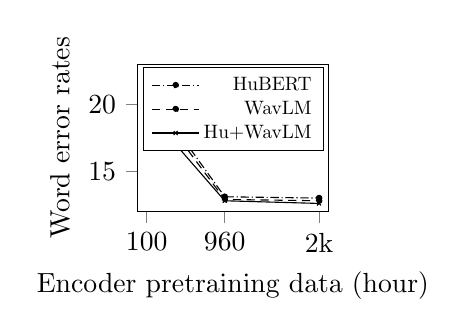
\begin{tikzpicture}
\begin{axis}[
    legend cell align={right},
    legend style={nodes={scale=0.7, transform shape}},
    width=0.33\textwidth,
    tick align=outside,
    tick pos=left,
    xlabel=Encoder pretraining data (hour),
    ylabel= Word error rates,
    xmin=0, xmax=2100,
    ymin=12, ymax=23,
    xtick={100,960, 2000},
    xticklabels={100,960, 2k},   % <---
    ytick={10,4,...,23}
            ]
\addplot[mark=*,black, mark size=1, densely dashdotted] 
plot coordinates {
    (100,21.2)
    (960,13.1)
    (2000,13.0)
};
\addlegendentry{HuBERT}

\addplot[color=black,mark=*, mark size=1, densely dashed]
    plot coordinates {
        (100,20.7)
        (960,12.9)
        (2000,12.8)
    };
\addlegendentry{WavLM}

\addplot[color=black,mark=x, mark size=1]
    plot coordinates {
        (100,19.5)
        (960,12.8)
        (2000,12.6)
    };
\addlegendentry{Hu+WavLM}
\end{axis}
%\caption{WER on test-other}
%\label{fig:werr_pretraining}
\end{tikzpicture}
% ---------------------------------------------------------------------------------------
\begin{tikzpicture}
\definecolor{darkgray176}{RGB}{176,176,176}
\begin{axis}[
legend cell align={left},
legend style={
    nodes={scale=0.7, transform shape},
  fill opacity=1.0,
  draw opacity=1.0,
  text opacity=1,
  at={(0.01,0.99)},
  anchor=north west,
  draw=none
},
width=0.33\textwidth,
tick align=outside,
tick pos=left,
x grid style={darkgray176},
xlabel={Encoder pre-training data (hour)},
xmin=-0.23, xmax=2.63,
xtick style={color=black},
xtick={0.2,1.2,2.2},
xticklabels={100,960,2k},
y grid style={darkgray176},
ylabel={Averaged WERR (\%)},
ymin=0, ymax=40.46875,
ytick style={color=black},
]
\draw[draw=black,fill=white,postaction={pattern=north east lines}] (axis cs:-0.1,0) rectangle (axis cs:0.1,2.08333333333334);
\draw[draw=black,fill=white,postaction={pattern=north east lines}] (axis cs:0.9,0) rectangle (axis cs:1.1,35.0694444444444);
\draw[draw=black,fill=white,postaction={pattern=north east lines}] (axis cs:1.9,0) rectangle (axis cs:2.1,36.1111111111111);
\addlegendimage{ybar,ybar legend,draw=black,fill=white,postaction={pattern=north east lines}}
\addlegendentry{HuBERT}

\draw[draw=black,fill=white,postaction={pattern=north west lines}] (axis cs:1.1,0) rectangle (axis cs:1.3,36.1111111111111);
\draw[draw=black,fill=white,postaction={pattern=north west lines}] (axis cs:2.1,0) rectangle (axis cs:2.3,37.5);
\draw[draw=black,fill=white,postaction={pattern=north west lines}] (axis cs:0.1,0) rectangle (axis cs:0.3,4.86111111111112);
\addlegendimage{ybar,ybar legend,draw=black,fill=white,postaction={pattern=north west lines}}
\addlegendentry{WavLM}


\draw[draw=black,fill=white,postaction={pattern=crosshatch}] (axis cs:1.3,0) rectangle (axis cs:1.5,37.5);
\draw[draw=black,fill=white,postaction={pattern=crosshatch}] (axis cs:2.3,0) rectangle (axis cs:2.5,38.5416666666667);
\draw[draw=black,fill=white,postaction={pattern=crosshatch}] (axis cs:0.3,0) rectangle (axis cs:0.5,9.375);
\addlegendimage{ybar,ybar legend,draw=black,fill=white,postaction={pattern=crosshatch}}
\addlegendentry{Hu+WavLM}

\end{axis}
%\caption{Relative WERRs}
\label{fig:werr_pretraining}
\end{tikzpicture}
% ---------------------------------------------------------------------------------------
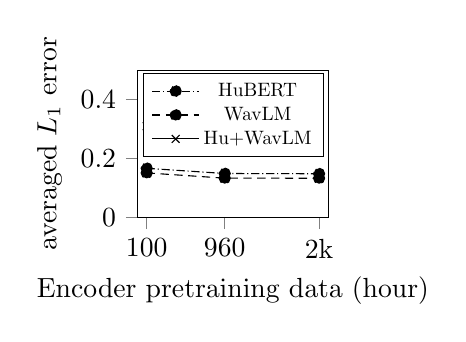
\begin{tikzpicture}
\begin{axis}[
    legend style={nodes={scale=0.7, transform shape}},
    width=0.33\textwidth,
    tick align=outside,
    tick pos=left,
    xlabel=Encoder pretraining data (hour),
    ylabel=averaged $L_1$ error,
    xmin=0, xmax=2100,
    ymin=0, ymax=0.5,
    xtick={100,960, 2000},
    xticklabels={100,960, 2k},   % <---
    ytick={0.1,0.05,...,0.4}
            ]
\addplot[mark=*,black, densely dashdotted] 
plot coordinates {
    (100,0.1667)
    (960,0.1490)
    (2000,0.1482)
};
\addlegendentry{HuBERT}

\addplot[color=black,mark=*, densely dashed]
    plot coordinates {
        (100,0.1511)
    (960,0.1332)
    (2000,0.13302)
    };
\addlegendentry{WavLM}

\addplot[color=black,mark=x]
    plot coordinates {
        (100,0.3095)
    (960,0.2988)
    (2000,0.2972)
    };
\addlegendentry{Hu+WavLM}
\end{axis}
%\caption{$L_1$ error}
\label{fig:l1_err_pretraining}
\end{tikzpicture}

    \begin{subfigure}[b]{.31\textwidth}
        \centering
        
\begin{tikzpicture}
\begin{axis}[
    legend cell align={right},
    legend style={nodes={scale=0.6, transform shape}},
    width=\textwidth,
    tick align=outside,
    tick pos=left,
    xlabel=Encoder pre-training data (hours),
    ylabel= WER (\%),
    xmin=0, xmax=2100,
    ymin=12, ymax=23,
    xtick={100,960, 2000},
    xticklabels={100,960, 2k},   % <---
    ytick={10,4,...,23}
            ]
\addplot[mark=*,black, mark size=1, densely dashdotted] 
plot coordinates {
    (100,21.2)
    (960,13.1)
    (2000,13.0)
};
\addlegendentry{Hu}

\addplot[color=black,mark=*, mark size=1, densely dashed]
    plot coordinates {
        (100,20.7)
        (960,12.9)
        (2000,12.8)
    };
\addlegendentry{WL}

\addplot[color=black,mark=x, mark size=1]
    plot coordinates {
        (100,19.5)
        (960,12.8)
        (2000,12.6)
    };
\addlegendentry{Hu+WL}
\end{axis}
\end{tikzpicture}

        \caption{WERs of student models.}
        \label{fig:WER pretraining 100h}
    \end{subfigure}
    \begin{subfigure}[b]{.31\textwidth}
    \centering
    % This file was created with tikzplotlib v0.10.1.

% to show only one bar in the legend
\pgfplotsset{compat=1.11,
    /pgfplots/ybar legend/.style={
    /pgfplots/legend image code/.code={%
       \draw[##1,/tikz/.cd,yshift=-0.25em]
        (0cm,0cm) rectangle (3pt,0.8em);},
   },
}
\begin{tikzpicture}
\definecolor{darkgray176}{RGB}{176,176,176}
\begin{axis}[
legend cell align={left},
legend style={
    nodes={scale=0.6, transform shape},
  % fill opacity=0.8,
  % draw opacity=1,
  % text opacity=1,
   ,
  anchor=north west,
  draw=none
},
width=\textwidth,
tick align=outside,
tick pos=left,
x grid style={darkgray176},
xlabel={Encoder pre-training data (hours)},
xmin=-0.23, xmax=2.63,
xtick style={color=black},
xtick={0.2,1.2,2.2},
xticklabels={100,960,2k},
y grid style={darkgray176},
ylabel={relative WERR (\%)},
ymin=0, ymax=41,
ytick style={color=black},
]
\draw[draw=black,fill=white,postaction={pattern=north east lines}] (axis cs:-0.1,0) rectangle (axis cs:0.1,2.08333333333334);
\draw[draw=black,fill=white,postaction={pattern=north east lines}] (axis cs:0.9,0) rectangle (axis cs:1.1,35.0694444444444);
\draw[draw=black,fill=white,postaction={pattern=north east lines}] (axis cs:1.9,0) rectangle (axis cs:2.1,36.1111111111111);
\addlegendimage{ybar,ybar legend,draw=black,fill=white,postaction={pattern=north east lines}}
\addlegendentry{Hu}

\draw[draw=black,fill=white,postaction={pattern=north west lines}] (axis cs:1.1,0) rectangle (axis cs:1.3,36.1111111111111);
\draw[draw=black,fill=white,postaction={pattern=north west lines}] (axis cs:2.1,0) rectangle (axis cs:2.3,37.5);
\draw[draw=black,fill=white,postaction={pattern=north west lines}] (axis cs:0.1,0) rectangle (axis cs:0.3,4.86111111111112);
\addlegendimage{ybar,ybar legend,draw=black,fill=white,postaction={pattern=north west lines}}
\addlegendentry{WL}


\draw[draw=black,fill=white,postaction={pattern=crosshatch}] (axis cs:1.3,0) rectangle (axis cs:1.5,37.5);
\draw[draw=black,fill=white,postaction={pattern=crosshatch}] (axis cs:2.3,0) rectangle (axis cs:2.5,38.5416666666667);
\draw[draw=black,fill=white,postaction={pattern=crosshatch}] (axis cs:0.3,0) rectangle (axis cs:0.5,9.375);
\addlegendimage{ybar,ybar legend,draw=black,fill=white,postaction={pattern=crosshatch}}
\addlegendentry{Hu+WL}

\end{axis}
\end{tikzpicture}
    \caption{Relative WERRs of student models.}
    \label{fig:WERR pretraining 100h}
    \end{subfigure}
    \begin{subfigure}[b]{.31\textwidth}
    \centering
    % This file was created with tikzplotlib v0.10.1.

\begin{tikzpicture}
\begin{axis}[
    legend style={nodes={scale=0.6, transform shape}},
    width=\textwidth,
    tick align=outside,
    tick pos=left,
    xlabel=Encoder pre-training data (hours),
    ylabel=averaged $L_1$ error,
    xmin=0, xmax=2100,
    ymin=0, ymax=0.48,
    xtick={100,960, 2000},
    xticklabels={100,960, 2k},   % <---
    ytick={0.1,0.05,...,0.4}
            ]
\addplot[mark=*,black, densely dashdotted] 
plot coordinates {
    (100,0.1667)
    (960,0.1490)
    (2000,0.1482)
};
\addlegendentry{Hu}

\addplot[color=black,mark=*, densely dashed]
    plot coordinates {
        (100,0.1511)
    (960,0.1332)
    (2000,0.13302)
    };
\addlegendentry{WL}

\addplot[color=black,mark=x]
    plot coordinates {
        (100,0.3095)
    (960,0.2988)
    (2000,0.2972)
    };
\addlegendentry{Hu+WL}
\end{axis}
\end{tikzpicture}
    \caption{$L_1$ error after pre-training.}
    \label{fig:l1 error}
    \end{subfigure}
    \caption{\%WERs and relative WERRs of student models pre-trained with different amount of acoustic data. All models were fine-tuned with the 100 hour ground truth data.}
    
\end{figure*}

\begin{table}[!ht]
    \centering
    \begin{tabular}{lcccc}
        \toprule
        \multirow{2}{*}{Teacher model}    & \multicolumn{2}{c}{dev}   & \multicolumn{2}{c}{test}  \\
        \cmidrule(lr){2-3}  \cmidrule(lr){4-5}
        & \multicolumn{1}{c}{clean} & \multicolumn{1}{c}{other} & \multicolumn{1}{c}{clean} & \multicolumn{1}{c}{other} \\ 
        \midrule
        \multicolumn{5}{l}{\textbf{100h fine-tune}}\\

        Hu  & 7.3 & 15.5 & 7.3 & 15.7 \\
        
        WL  & 6.8 & 15.3 & 7.2 & 15.3 \\
        
        WL+Hu  & 6.8 & 15.0 & 7.0 & 15.2 \\
        \midrule
        \multicolumn{5}{l}{\textbf{960h fine-tune}}\\
        
        Hu & 4.6 & 9.4 & 4.6 & 9.7 \\
        WL & 4.1 & 9.2 & 4.2 & 9.2 \\
        WL+Hu  & 3.8 & 8.8 & 3.9 & 9.0 \\
        
        \bottomrule
    \end{tabular}
    \caption{\%WERs for non-streaming student transducer models pre-trained on 2k hours. Only embedding KD is adopted.}
    \label{tab:extra unlabelled}
\end{table}

To investigate if extra unlabelled data from another domain helps embedding-level KD, the extra 1000 hours of unlabelled data from Libri-Light was incorporated during encoder KD training for non-streaming student models. Fine-tuning with train-clean-100 ground truth data and 960 hours mix data are carried out and the WERs are shown in \tbl{extra unlabelled}. 
Compared to the result in \tbl{feature kd 960h}, the WERs were further improved after increasing the pre-training dataset from 960 to 2k hours.

\subsection{Pretraining Error and Finetuning Accuracy}

%To further exploit unlabelled data, the 1000 hour randomly sampled audio from Libri-Light is incorporated during encoder pre-training.
The previous experiments demonstrated that the student model achieves better performance with the increase of pre-training data, indicating that a better encoder initialisation is learned in the first stage. Apart from the WER after fine-tuning, the KD training in the first stage can also be evaluated with the $L_1$ error on test sets. Here, the relationship between the $L_1$ error after pre-training and the final WER is investigated. The fine-tuning results of the student models pre-trained with 100 hours, 960 hours and 2k hours data are shown in \figdot{WER pretraining 100h} and \figdot{WERR pretraining 100h}. Note that only train-clean-100 is used during fine-tuning.
% The result of encoder pre-training can be evaluated by the $L_1$\figdot{WER pretraining} and \figdot{WERR pretraining} show the student model's WERs on test-other with different amount of encoder pre-training data and their corresponding WERRs compared to the baseline model trained on 100h. Fine-tuning with both 100 hour and 860 hour text-audio pair are experimented. The WERs decrease as the amount of encoder pre-training data increases, suggesting that the encoder learns a better initialisation with extra unlabelled data. 

The normalised $L_1$ error on the development set of student models pre-trained with different amounts of unlabelled data is illustrated in \figdot{l1 error}. The $L_1$ error decreases with extra unlabelled data used during encoder pre-training for both the single-teacher and multi-teacher setups. This is in-line with the improved student model performance after fine-tuning. However, a lower $L_1$ error does not guarantee a better student model after fine-tuning when comparing single-teacher and multi-teacher setups (see \figdot{WERR pretraining 100h}). The student model trained with two teachers (HuBERT and WavLM) has a much higher $L_1$ error than the single-teacher setup, but yields lower WERs after fine-tuning. This could be the reason that the random teacher model selection strategy drives the encoder initialisation to a manifold that is in between the teacher models and can be quickly adapted to the fine-tuning data. This also effectively prevents the student model from overfitting to a single teacher, which is beneficial for multi-teacher training.

% \begin{figure}
%     \centering
%     % This file was created with tikzplotlib v0.10.1.

\begin{tikzpicture}
\begin{axis}[
    legend style={nodes={scale=0.6, transform shape}},
    width=\textwidth,
    tick align=outside,
    tick pos=left,
    xlabel=Encoder pre-training data (hours),
    ylabel=averaged $L_1$ error,
    xmin=0, xmax=2100,
    ymin=0, ymax=0.48,
    xtick={100,960, 2000},
    xticklabels={100,960, 2k},   % <---
    ytick={0.1,0.05,...,0.4}
            ]
\addplot[mark=*,black, densely dashdotted] 
plot coordinates {
    (100,0.1667)
    (960,0.1490)
    (2000,0.1482)
};
\addlegendentry{Hu}

\addplot[color=black,mark=*, densely dashed]
    plot coordinates {
        (100,0.1511)
    (960,0.1332)
    (2000,0.13302)
    };
\addlegendentry{WL}

\addplot[color=black,mark=x]
    plot coordinates {
        (100,0.3095)
    (960,0.2988)
    (2000,0.2972)
    };
\addlegendentry{Hu+WL}
\end{axis}
\end{tikzpicture}
%     \caption{Averaged L1 error after encoder pre-training with different teacher setups and different amount of data.}
%     \label{fig:l1 error}
% \end{figure}



% \begin{figure}[!h]
%     \centering
%     \includegraphics[width=.8\linewidth]{figs/l1_error.pdf}
%     \caption{$L_1$ error of after encoder pre-training with different amount of data.}
%     \label{fig:l1 error}
% \end{figure}

% ============================
% \begin{table}[H]
%     \centering
%     \begin{tabular}{lcccc}
%         \toprule
%         \multirow{2}{*}{Transducer models}    & \multicolumn{2}{c}{dev}   & \multicolumn{2}{c}{test}  \\
%         \cmidrule(lr){2-3}  \cmidrule(lr){4-5}
%         & \multicolumn{1}{c}{clean} & \multicolumn{1}{c}{other} & \multicolumn{1}{c}{clean} & \multicolumn{1}{c}{other} \\ 
%         \midrule
%         \multicolumn{5}{l}{\textbf{100h finetuning}} \\
%         100 \\
%         960 \\
%         2k \\
        
%         \midrule
%         \multicolumn{5}{l}{\textbf{960h finetuning}} \\
%         100 \\
%         960 \\
%         2k \\
        
%         \bottomrule
%     \end{tabular}
%     \caption{WERs for non-streaming student transducer models pre-trained with different amount of unlabelled data}
%     \label{tab:feature kd 960h}
% \end{table}
